% AUTO-GENERATED durch diagram_generator (P3, Config-Streuungs-ECDF; lang=de)
% EHRLICH: Population = die KONFIGURATIONEN (Permutationen), jede = 1 ns_per_op-Punkt. Das ist die
% Verteilung UEBER die Konfigurationen (Anteil der Configs mit Latenz <= x), NICHT eine Per-Operation-
% Latenz-CDF (die rohen Einzel-Op-Latenzen traegt das WIDE-Schema nicht). 1 Treppe je search_algo.
\begin{figure}[!htbp]
\centering
\resizebox{\textwidth}{!}{%
\begin{tikzpicture}
\begin{axis}[
    width=0.7800\textwidth,
    height=0.4000\textheight,
    scale only axis,
    title={ECDF der Gesamt-Latenz - Verteilung ueber Konfigurationen},
    xlabel={Gesamt-Latenz je Konfiguration ns\_per\_op (ns, log)},
    ylabel={Anteil der Konfigurationen mit Latenz <= x},
    grid=both,
    enlargelimits=0.05,
    xmode=log,
    ymin=0, ymax=1,
    legend pos=south east,
    legend style={font=\tiny,legend cell align=left},
]
\addplot+[const plot,mark=none,thick] coordinates {
    (671.5320,0)
    (671.5320,1.0000)
};
\addlegendentry{k\_ary (N=1)}
\end{axis}
\end{tikzpicture}
}%
\caption{ECDF der Gesamt-Latenz - Verteilung ueber Konfigurationen}
\end{figure}
